\chapter{Introduction}
\label{cha:introduction}
This chapter gives a brief overview of the the document's overall motivation, its current state and the needed background knowledge that is required to read this document.

\section{Motivation and current state}
As the title suggests, the document's overall motivation is to deliver a subject-oriented approach of a git manual.
Git is a Version Control System (VCS) developed by Linus Torvalds \cite{LM12}. Compared to other VCSs, The main difference of git is that it has a different approach to file versioning and collaboration development, as both are much more efficient in git \cite{CS20}.
This makes git one of the most popular VCS out there, which is why the provision of git instruction is of particular interest.
The end goal of this document is to provide the \textit{ultimate} git manual. Its final version should aspire to provide all the necessary knowledge about git to any reader, regardless of his/her technical background.

As of the document's current state, it provides 12 git commands which lay a solid foundation for any basic git workflow. With the provided commands, the reader is able to: 
\begin{itemize} [nosep]
    \item \textbf{create} a git repository (\ref{sec:git_init})
    \item \textbf{add} (\ref{sec:git_add}) and \textbf{commit} (\ref{sec:git_commit}) any file within a git repository
    \item \textbf{check the current state} of a git repository at any given time (\ref{sec:git_status})
    \item \textbf{view} all existing branches and \textbf{create} new ones (\ref{sec:git_branch})
    \item \textbf{switch} to any existing branch (\ref{sec:git_checkout})
    \item \textbf{merge} different branches of a git repository (\ref{sec:git_merge})
    \item \textbf{set a new branch beginning} for any branch of a git repository (\ref{sec:git_rebase})
    \item \textbf{save} a copy of a remote git repository into the local storage (\ref{sec:git_clone})
    \item \textbf{fetch} commits of a remote repository (\ref{sec:git_fetch})
    \item \textbf{pull} (fetch and apply) commits of a remote repository on any branch (\ref{sec:git_pull})
    \item \textbf{push} commits of any branch of a repository to its local counterpart (\ref{sec:git_push})
\end{itemize}
This set of commands is enough for the majority of git workflows as the conjunction of all commands enables the usage of git's VCS functionality (\ref{cha:git_basics}), as well as the basic functionalities of branching (\ref{cha:git_branching}) and collaborations (\ref{cha:git_collaboration}).

\section{Foundations and related work}
There are three concepts that are required to fully understand this manual. The first concept is that git has introduced three different states for a file residing in a git repository.
\begin{figure} [H]
    \centering
    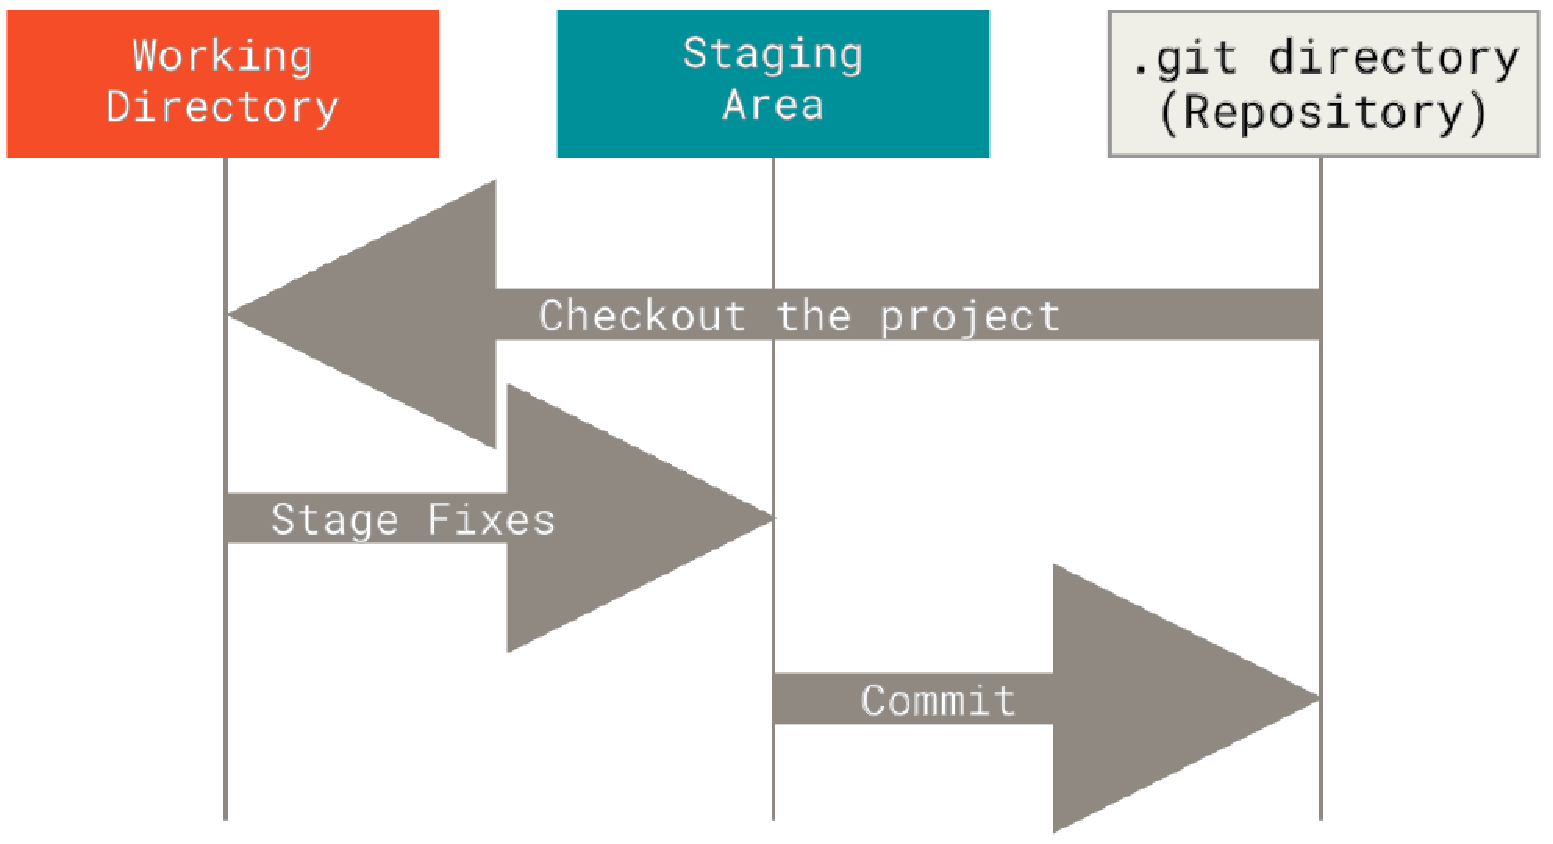
\includegraphics[width=\textwidth]{git_manual/figures/three_states.pdf}
    \caption{These are the transitions that happen in a state change\cite{CS20}}
    \label{fig:three_states}
\end{figure}
The three states are: \textit{modified}, \textit{staged} and \textit{committed}. If a file is modified, it means that the file has been changed or worked on, but is not committed yet.
To do that, the file has to be staged first. This means that the modified file is marked to go into the next commit. The file which keeps track of the marked files is called the \dq{}index\dq{}. If the user commits the staged file, the file is in its committed state which means that the data, containing the changes, is safely stored in the git repository

As seen in \ref{fig:three_states}, there are three locations the files can be in during the work with a git repository: the \textit{working directory}, \textit{staging area} and \textit{.git directory}. This is the second concept to remember during the read of the manual.
By opening any file within a git repository, git will automatically checkout the latest version of the project by translating and putting the compressed files within the repository onto the local disk. These modified files will then go through the three states depending on the workflow.

The third concept is completely unrelated to git and revolves around the process modeling schema itself. In the scope of this document, the Parallel Activity Specification Schema (PASS) is used to give a subject-oriented perspective of what process are involved during the interaction of a git user and the git software. Both are used as the main subjects of all Subject Interaction Diagrams (SID). Each git command has at least one SID. More details about PASS and its properties are found here \cite{El21}.
Here are some detailed descriptions of the main subjects:
\begin{itemize} [nosep]
    \item \textbf{Git User}: The Git User is the user of the git software.
    \item \textbf{Git UI + Software}: The Git UI could be the terminal of the user's current operating system or a graphical user interface written by a third party, such as GIT Bash. The git software is the actual part, which is installed in the user's computer. It contains all the logical operations required for the git commands.
\end{itemize}

\section{Outlook}
This is a list of git commands that are still left to model to complete the git manual in such a way so that its completed. However, this list does not contain every git command that is missing as each git command is heavily overloaded. An intrinsically complete manual is not only confusing, but unnecessary too as some overloaded git commands can be replaced with a sequence of other git commands.
\begin{itemize} [nosep]
    \item git config - Used to setup a profile for the git user, who contributes something to the 
    \item .gitignore: not a git command. However, it is important for the setup as the file is used to ignore unrelated files from the repository, e.g., .DS\_Store
    \item git diff: To see what has been modified which hasn't been staged yet
    \item git rm: removes a file from the git repository
    \item git log: views all commits
    \item git branch -d and git branch -D: deletes the targeted branch
    \item git cherry-pick: take a commit from a different branch and reintroduce it as new commit in the current branch
    \item git revert: take a commit from the current branch, remove it and introduce the removal as new commit. This essentially undoes the changes of the targeted commit.
    \item git stash: saves modified files on the computers stack. This is not a commit.
    \item git stash apply: Applies the modifications stored in the stash on the current branch again
    \item git stash list: Lists out all of the applicable stashes.
    \item git stash drop: Deletes the stashed modification from the stack.
    \item git reset: resets the HEAD pointer to a specific state.
    \item git push --set-upstream: pushes branches that are non existent in the remote repository into the remote repository.
\end{itemize}
After this list of commands is modeled completely, almost every functionality of git is unlocked and supported by this manual. The commands, which are intentionally left out, are rarely used even by professional software developers. However, if a git expert considers some commands missing, please refer to \cite{CS20} for guidance.